\section{Code-Snippets}

\subsection{iostream}
    \lstinputlisting{code/iostream.cpp}

\subsection{Einfaches Limit-Programm}
    Limit eingeben, anschliessend Summe aller Zahlen teilbar durch 3 und 7 ausgeben
    \lstinputlisting{code/rechnung_limit.cpp}

\subsection{Manuelle Allokation}\label{Manuelle Allokation}
    \lstinputlisting{code/manual_allocation.cpp}



\subsection{Memorymap}
    \lstinputlisting{code/memory-snippet.cpp}
    \nextcol
    \lstinputlisting{code/memory-snippet.h}
    \lstinputlisting{code/memory-snippet-main.cpp}

    \begin{center}
        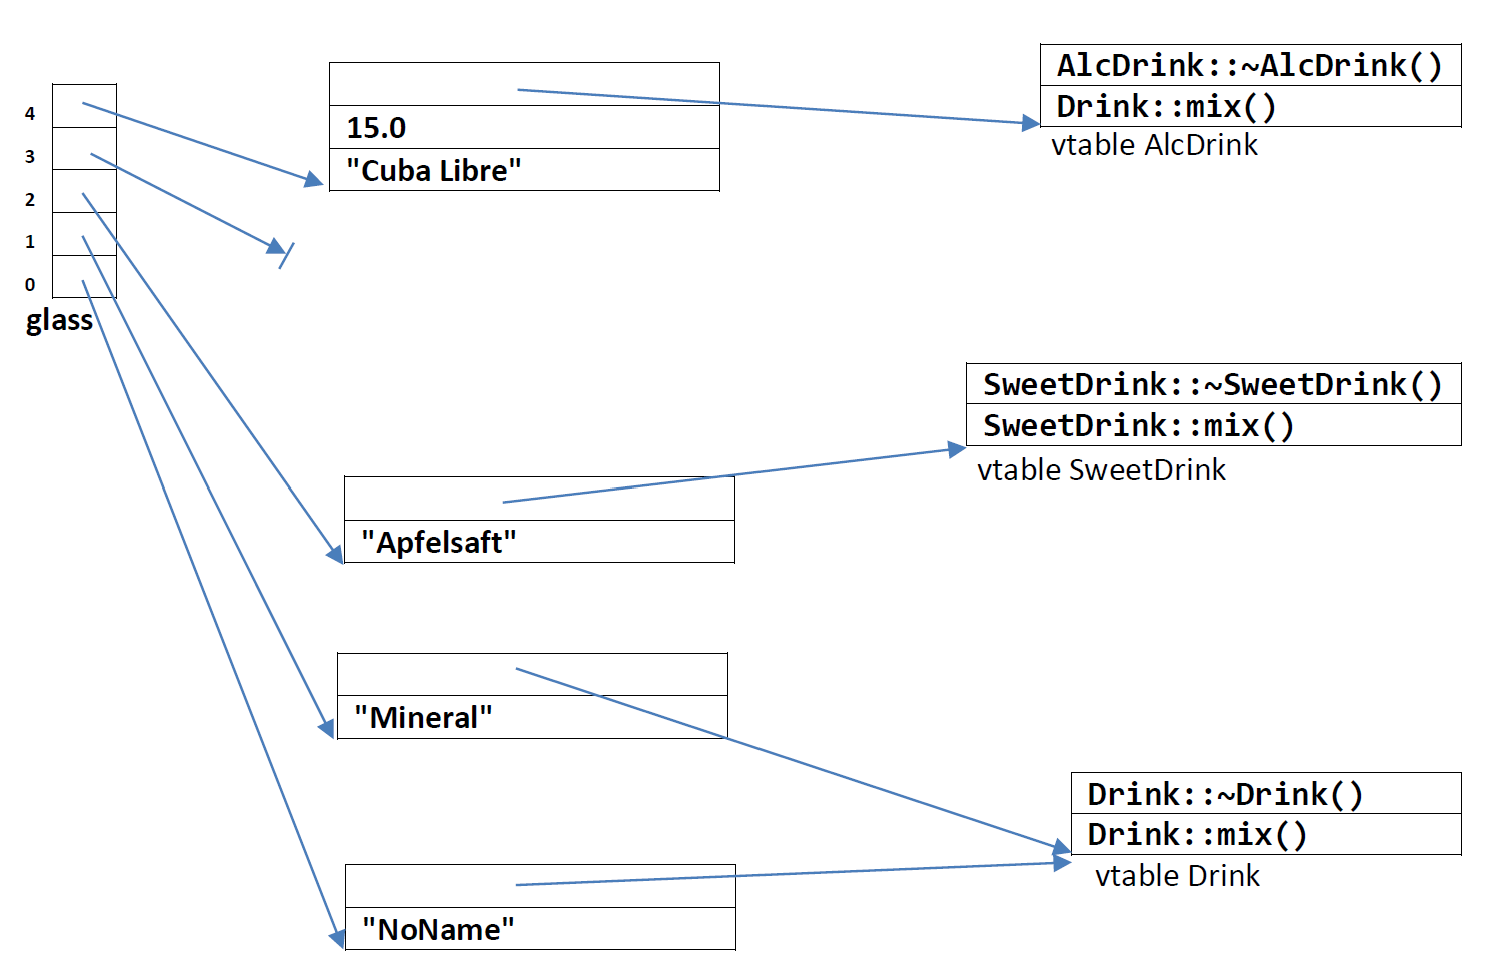
\includegraphics[width=\columnwidth]{pictures/memorymap-drink.png}  
    \end{center}
    \nextcol

\subsection{Templates}\label{Templates}
    Template für \verb|int sumOfElements(int* array, size_t size);|
    \lstinputlisting{code/templates_snippet.h}

\subsection{Overloading in Streams}
    \lstinputlisting{code/overloading-snippet.cpp}

    \nextcol

\subsection{Klassendiagramm Umsetzung}
    \begin{center}
        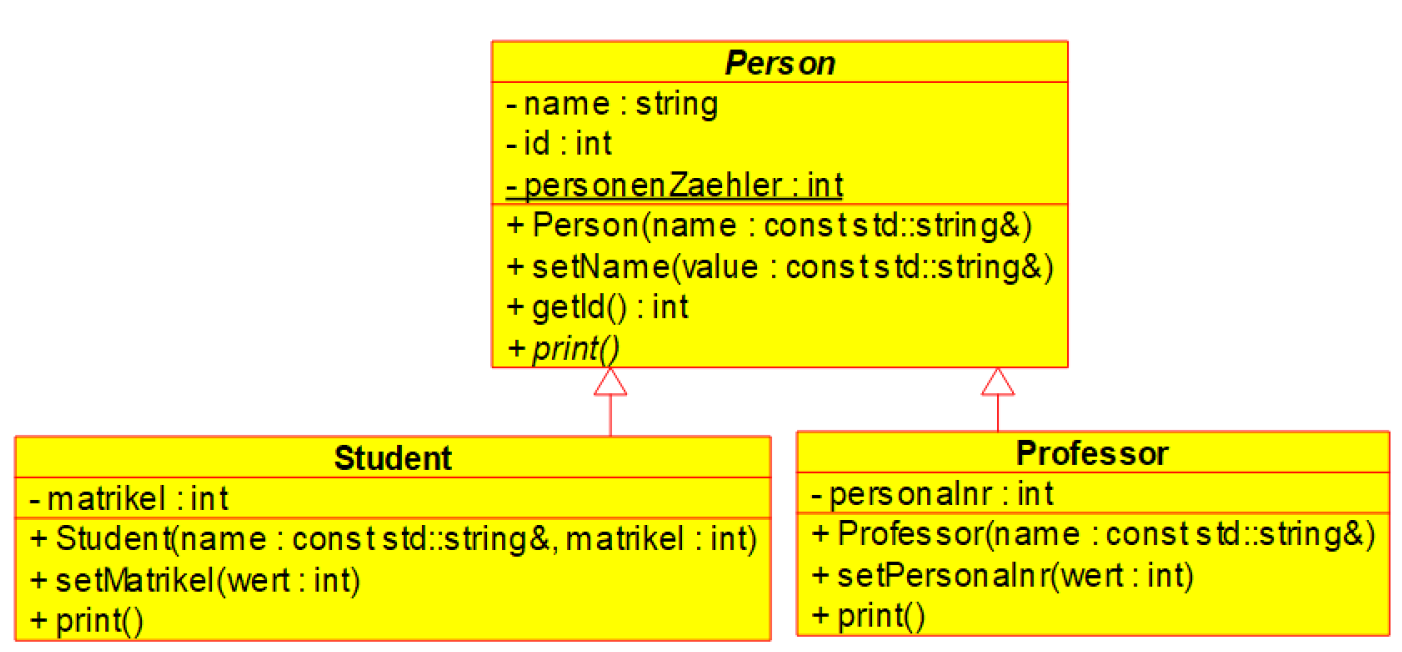
\includegraphics[width=\columnwidth]{pictures/Klassendiagramm-Umsetzung.png}
    \end{center}

    \lstinputlisting{code/classdiagram.h}

    \nextcol